%%%%%%%%%%%%%%%%%%%%%%%%%%%%%%%%%%%%%%%%%%%%%%%%%%%%%%%%%%%%%%%%%%%%%%%%%%%%%%%%%%%%%%%%%%%%%%%%%%%
%%%%%%%%%%%%%%%%%%%%%%%%%%%%%%%%%%%%%%%%%%%%%%%%%%%%%%%%%%%%%%%%%%%%%%%%%%%%%%%%%%%%%%%%%%%%%%%%%%%
%%%%%%%%%%%%%%%%%%%%%%%%%%%%%%%%%%%%%%%%%%%%%%%%%%%%%%%%%%%%%%%%%%%%%%%%%%%%%%%%%%%%%%%%%%%%%%%%%%%
%%%%%%%%%%%%%%%%%%%%%%%%%%%%%%%%%%%%%%%%%%%%%%%%%%%%%%%%%%%%%%%%%%%%%%%%%%%%%%%%%%%%%%%%%%%%%%%%%%%

\section{Conceptos}

Para poder identificar marcadores significativos para el diagnóstico del deterioro cognitivo, 
éste debe ser estudiado desde la neuropsicología; dentro de ésta última se destaca la técnica de 
electroencefalografía, que es usada para medir cierto tipo de actividad cerebral y que posiblemente 
esté asociada al deterioro cognitivo. 
Una vez expuestos los conceptos pertinentes, se presenta una colección de objetos matemáticos
(procesos estocásticos débilmente estacionarios) con los cuales se han modelado un tipo de
actividad cerebral, y que fue comparado con mediciones de la misma.

La exposición se divide en dos subsecciones marcadamente diferentes: matemáticas y 
fisiología/psicología.
En la primera se menciona al deterioro cognitivo en adultos mayores, con énfasis en su 
caracterización dentro del sistema nervioso.
La segunda subsección se centra en las herramientas estadísticas utilizadas para analizar datos 
experimentales, entendidas no como simples \textit{técnicas} sino como objetos abstractos
definidos formalmente.

Estas dos partes difieren no sólo en temas sino también epistemológicamente: en la
primera aparecen afirmaciones basadas en datos experimentales, acompañadas de las citas 
pertinentes, mientras que en la segunda las
afirmaciones son formalmente verdaderas y demostrables en el sistema 
axiomático usual. Respecto a estas últimas, varias de las demostraciones se presentan como 
apéndice junto las definiciones pertinentes, mientras otras son citadas debido a diversos motivos.

\subsection{Psicología}

%La demencia es un síndrome debido a la disfunción cerebral, que produce desintegración
%de la conducta en los planos intelectual y emocional, alterando significativamente la
%función social y laboral del paciente.

La \textbf{demencia} es, según el Manual diagnóstico de y estadístico de trastornos mentales
(DSM-IV), \textit{un síndrome que consiste en el desarrollo de déficit cognoscitivos
suficientemente graves como para interferir significativamente en las actividades laborales 
y sociales, respecto al nivel de actividad previo. 
%Aparece precedida por una enfermedad médica o
%el efecto de exposición prolongada a sustancias tóxicas, incluso ambos.
Los sujetos con demencia tienen una baja capacidad para aprender información nueva y 
suelen olvidar lo aprendido anteriormente, siendo éste el síntoma más prominente} \cite{DCM_5}.

Cuando un sujeto presenta cambios marcados en su conducta, es relativamente fácil identificar
la demencia; caso contrario es el diagnóstico temprano de la misma, el cual es importante
para un tratamiento adecuado que 
revierta o desacelere el avance de este síndrome.
Se ha señalado que los criterios del manual DSM-IV son suficientes para este diagnóstico
\cite{Knopman01}.


Considerando a los \textbf{adultos mayores}, entendidos como individuos de 60 años o más,
conviene destacar que el
envejecimiento es determinado por una serie de procesos moleculares, celulares, fisiológicos y 
psicológicos que conducen directamente al deterioro de funciones cognitivas, específicamente 
atención y memoria \cite{Navarrete03,Park09}.
%Aunque popularmente se asocia a la vejez con el deterioro cognitivo,
La funcionalidad durante esta etapa se relaciona con el estilo de vida, los factores de riesgo, el 
acceso a la educación y las acciones para el cuidado de la salud realizadas en edades más 
tempranas \cite{Ohayon04,Sanhueza14}.
%En un principio, se consideraba que el envejecimiento cerebral ocurr\'ia fundamentalmente por una 
%muerte neuronal \cite{Coleman87}, sin embargo, estudios realizados con tejido cerebral post mortem 
%de adultos mayores que en vida fueron sanos, mostraron que dicha muerte neuronal no alcanza un 10\% 
%del tejido \cite{Esiri07}. 

%Con el paso del tiempo, la organizaci\'on an\'atomo-funcional del cerebro sufre modificaciones que 
%traen como consecuencia la afectaci\'on de diferentes capacidades cognitivas; sin embargo, la 
%vulnerabilidad de los circuitos neuronales ante estos cambios no suceden de forma homog\'enea en 
%todo el cerebro \cite{Hita14}.

Al momento de diagnosticar deterioro cognitivo en adultos mayores, deben tenerse en cuenta
el envejecimiento normal y la posible \textbf{pseudodemencia depresiva}, ya que presentan
características similares. Con respecto a ésta última, definida como \textit{un
trastorno del afecto y que produce un aparente deterioro cognitivo} \cite{DCM_5},
aunque no es efectivamente un tipo de demencia bien puede desencadenar en ello
en ausencia de un tratamiento adecuado.

Como es usual, se considerará como etapa precursora de la demencia al
\textbf{deterioro cognitivo leve}, definido como \textit{un
síndrome caracterizado por una alteración adquirida y prolongada de una o varias funciones 
cognitivas, que no corresponde a un síndrome focal y no cumple criterios suficientes de 
gravedad para ser calificada como demencia} \cite{Robles02}.
En el transcurso de este escrito este padecimiento
será manejado como \textbf{posible deterioro cognitivo (PDC)} ya
que el autor no tiene la autoridad ni la autorización para efectuar un diagnóstico clínico, y 
porque los síntomas en esta etapa se consideran --afortunadamente-- reversibles.


\subsubsection{Diagnóstico de la demencia}

En psicología los instrumentos de medición estándar son las \textbf{pruebas neuropsicológicas}, 
entendidas como muestras
de alguna conducta de interés a las que se asignan puntajes para comparar cuantitativamente
entre sujetos \cite{Ardila12}.

Las habilidades medibles a través de test neuropsicológicas se suelen agrupar en áreas o
\textbf{dominios}: atención, lenguaje, cálculo, memoria y aprendizaje, percepción,
motricidad, funciones somatosensoriales, habilidades espaciales, funciones ejecutivas. 
%Principales sindromes neuropsicologicos
%Afasia 
%Alexia 
%Agrafia 
%Acalculia 
%Agnosia 
%Apraxia 
%Amnesia 
%Sindrome disejecutivo 
%Demencia
%No  existe  un  manual  de  síndromes  neuropsicológicos,  aunque  muchos  de  ellos  se incluyen 
%en el Manual Diagnóstico y Estadístico de los Trastornos Mentales (DSM-IV, 1994)  y  en  la 
%Clasificación  Internacional  de  las  Enfermedades (ICD-10,  World  Health Organization, 2007).

HACER, QUIZA, UN CUADRO SOBRE LOS DOMINIOS Y SUS RELACIONES CON LAS PARTES DEL CEREBRO

%%%%%%%%%%%%%%%%%%%%%%%%%%%%%%%%%%%%%%%%%%%%%%%%%%%%%%%%%%%%%%%%%%%%%%%%%%%%%%%%%%%%%%%%%%%%%%%%%%%
%%%%%%%%%%%%%%%%%%%%%%%%%%%%%%%%%%%%%%%%%%%%%%%%%%%%%%%%%%%%%%%%%%%%%%%%%%%%%%%%%%%%%%%%%%%%%%%%%%%

\subsection{Fisiología}

El sistema nervioso central consiste en la médula espinal y el cerebro, siendo el segundo una
porción altemente especializada del primero; aparece protegido por las meninges, un grpo de tres capas 
protectoras, e inmerso en el llamado líquido cefalorraquídeo.
El cerebro se divide en tres partes: tallo cerebral, cerebelo y hemisferios cerebrales;
éstos últimos tienen asociadas las llamadas \textit{funciones superiores}, como son uso de lenguaje,
reconocimiento de rostros, aprendizaje, conciencia, etc., por lo que se les prestará
atención de forma exclusiva.

Los hemisferios cerebrales se componen de capas, de las cuales la más externa se conoce como
\textit{corteza cerebral}; tiene cerca de 1 cm de espesor y un color grisáceo debido a que
las céulas nerviosas en esa capa están muy densamente emapquetadas, y debido a lo cual se le conoce
como \textit{materia gris}.

La corteza cerebral presenta numerosos pliegues organizados en \textit{giros} (crestas) y
\textit{surcos} (valles), los surcos más profundos se llaman \textit{fisuras} y son usados
como referencia;
la fisura lateral define al \textbf{lóbulo temporal} como la porción por debajo de 
éste, mientras que la fisura central define al \textbf{lóbulo frontal} como la
porción delante de éste (ver figura \ref{lobulos}). Los \textbf{lóbulos parietal y occipital}
se encuentran, respectivamente, detrás de los lóbulos frontal y temporal.

Varias de las funciones superiores han sido asociadas con 

\begin{figure}
\centering
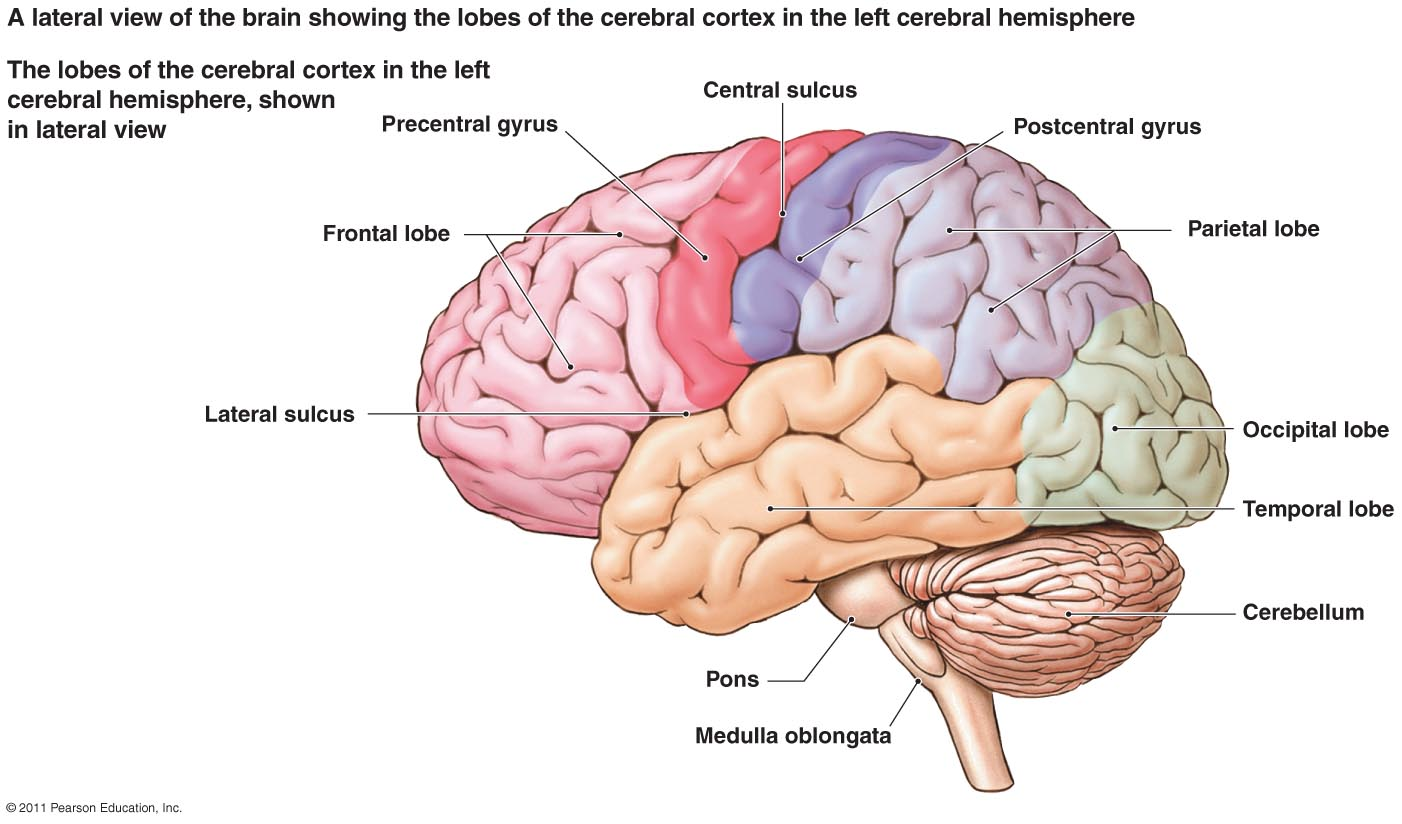
\includegraphics[width=0.8\linewidth]{./img_diagramas/brainlandmarks.jpg} 
\caption{Referentes fisiológicos usadas para definir a los lóbulos cerebrales.
Este gráfico será redibujado.
}
\label{lobulos}
\end{figure}

\begin{figure}
\centering
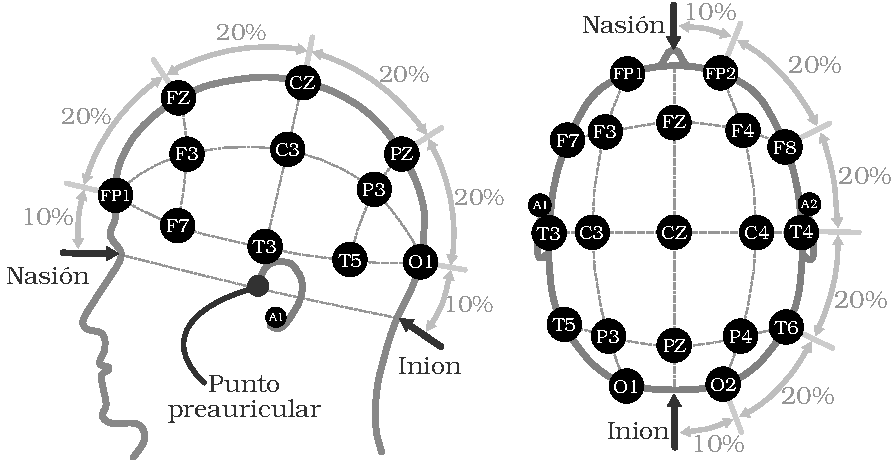
\includegraphics[width=\linewidth]{./img_diagramas/cabeza_proporcionada.pdf} 
\caption{Colocación de electrodos según el sistema 10--20. El \textbf{inion} es 
una protuberancia craneal, mientras que el \textbf{nasión} es la unión del hueso frontal y los 
huesos nasales; el \textbf{punto preauricular} se ubica arriba del cartílago llamado tragus, que 
protege el canal auditivo \cite{Butkov07}. 
}
\label{img1020}
\end{figure}

\begin{figure}
\centering
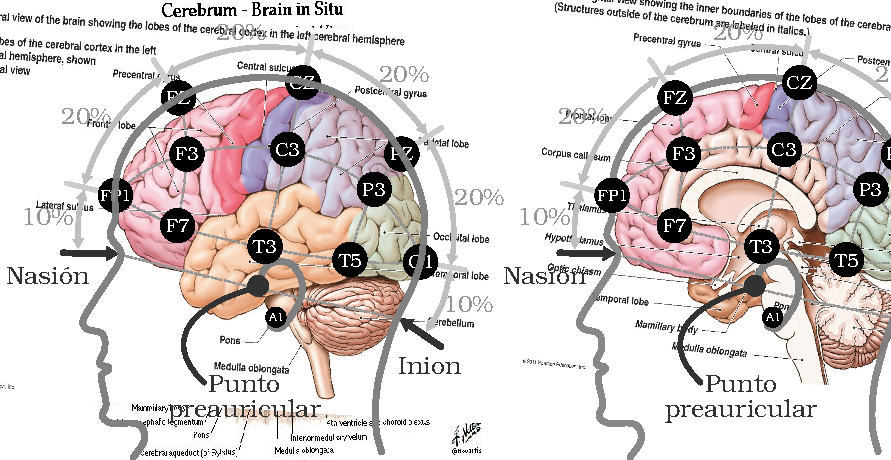
\includegraphics[width=\linewidth]{./img_diagramas/cerebro_1020.pdf} 
\caption{Esquema de la correspondencia entre el Sistema 10-20 y las regiones de la corteza
cerebral que representan, aproximadamente. Este gráfico será reconstruido.
}
\label{corresponde_1020}
\end{figure}

%%%%%%%%%%%%%%%%%%%%%%%%%%%%%%%%%%%%%%%%%%%%%%%%%%%%%%%%%%%%%%%%%%%%%%%%%%%%%%%%%%%%%%%%%%%%%%%%%%%
%%%%%%%%%%%%%%%%%%%%%%%%%%%%%%%%%%%%%%%%%%%%%%%%%%%%%%%%%%%%%%%%%%%%%%%%%%%%%%%%%%%%%%%%%%%%%%%%%%%

\subsection{Sueño}

%textwidth: \printinunitsof{cm}\prntlen{\textwidth}
%
%linewidth: \printinunitsof{cm}\prntlen{\linewidth}

%%%%%%%%%%%%%%%%%%%%%%%%%%%%%%%%%%%%%%%%%%%%%%%%%%%%%%%%%%%%%%%%%%%%%%%%%%%%%%%%%%%%%%%%%%%%%%%%%%%
%%%%%%%%%%%%%%%%%%%%%%%%%%%%%%%%%%%%%%%%%%%%%%%%%%%%%%%%%%%%%%%%%%%%%%%%%%%%%%%%%%%%%%%%%%%%%%%%%%%
%%%%%%%%%%%%%%%%%%%%%%%%%%%%%%%%%%%%%%%%%%%%%%%%%%%%%%%%%%%%%%%%%%%%%%%%%%%%%%%%%%%%%%%%%%%%%%%%%%%
%%%%%%%%%%%%%%%%%%%%%%%%%%%%%%%%%%%%%%%%%%%%%%%%%%%%%%%%%%%%%%%%%%%%%%%%%%%%%%%%%%%%%%%%%%%%%%%%%%%
